\documentclass[twoside]{book}

% Packages required by doxygen
\usepackage{fixltx2e}
\usepackage{calc}
\usepackage{doxygen}
\usepackage[export]{adjustbox} % also loads graphicx
\usepackage{graphicx}
\usepackage[utf8]{inputenc}
\usepackage{makeidx}
\usepackage{multicol}
\usepackage{multirow}
\PassOptionsToPackage{warn}{textcomp}
\usepackage{textcomp}
\usepackage[nointegrals]{wasysym}
\usepackage[table]{xcolor}

% Font selection
\usepackage[T1]{fontenc}
\usepackage[scaled=.90]{helvet}
\usepackage{courier}
\usepackage{amssymb}
\usepackage{sectsty}
\renewcommand{\familydefault}{\sfdefault}
\allsectionsfont{%
  \fontseries{bc}\selectfont%
  \color{darkgray}%
}
\renewcommand{\DoxyLabelFont}{%
  \fontseries{bc}\selectfont%
  \color{darkgray}%
}
\newcommand{\+}{\discretionary{\mbox{\scriptsize$\hookleftarrow$}}{}{}}

% Page & text layout
\usepackage{geometry}
\geometry{%
  a4paper,%
  top=2.5cm,%
  bottom=2.5cm,%
  left=2.5cm,%
  right=2.5cm%
}
\tolerance=750
\hfuzz=15pt
\hbadness=750
\setlength{\emergencystretch}{15pt}
\setlength{\parindent}{0cm}
\setlength{\parskip}{3ex plus 2ex minus 2ex}
\makeatletter
\renewcommand{\paragraph}{%
  \@startsection{paragraph}{4}{0ex}{-1.0ex}{1.0ex}{%
    \normalfont\normalsize\bfseries\SS@parafont%
  }%
}
\renewcommand{\subparagraph}{%
  \@startsection{subparagraph}{5}{0ex}{-1.0ex}{1.0ex}{%
    \normalfont\normalsize\bfseries\SS@subparafont%
  }%
}
\makeatother

% Headers & footers
\usepackage{fancyhdr}
\pagestyle{fancyplain}
\fancyhead[LE]{\fancyplain{}{\bfseries\thepage}}
\fancyhead[CE]{\fancyplain{}{}}
\fancyhead[RE]{\fancyplain{}{\bfseries\leftmark}}
\fancyhead[LO]{\fancyplain{}{\bfseries\rightmark}}
\fancyhead[CO]{\fancyplain{}{}}
\fancyhead[RO]{\fancyplain{}{\bfseries\thepage}}
\fancyfoot[LE]{\fancyplain{}{}}
\fancyfoot[CE]{\fancyplain{}{}}
\fancyfoot[RE]{\fancyplain{}{\bfseries\scriptsize Generated by Doxygen }}
\fancyfoot[LO]{\fancyplain{}{\bfseries\scriptsize Generated by Doxygen }}
\fancyfoot[CO]{\fancyplain{}{}}
\fancyfoot[RO]{\fancyplain{}{}}
\renewcommand{\footrulewidth}{0.4pt}
\renewcommand{\chaptermark}[1]{%
  \markboth{#1}{}%
}
\renewcommand{\sectionmark}[1]{%
  \markright{\thesection\ #1}%
}

% Indices & bibliography
\usepackage{natbib}
\usepackage[titles]{tocloft}
\setcounter{tocdepth}{3}
\setcounter{secnumdepth}{5}
\makeindex

% Hyperlinks (required, but should be loaded last)
\usepackage{ifpdf}
\ifpdf
  \usepackage[pdftex,pagebackref=true]{hyperref}
\else
  \usepackage[ps2pdf,pagebackref=true]{hyperref}
\fi
\hypersetup{%
  colorlinks=true,%
  linkcolor=blue,%
  citecolor=blue,%
  unicode%
}

% Custom commands
\newcommand{\clearemptydoublepage}{%
  \newpage{\pagestyle{empty}\cleardoublepage}%
}

\usepackage{caption}
\captionsetup{labelsep=space,justification=centering,font={bf},singlelinecheck=off,skip=4pt,position=top}

%===== C O N T E N T S =====

\begin{document}

% Titlepage & ToC
\hypersetup{pageanchor=false,
             bookmarksnumbered=true,
             pdfencoding=unicode
            }
\pagenumbering{alph}
\begin{titlepage}
\vspace*{7cm}
\begin{center}%
{\Large Game \\[1ex]\large 1 }\\
\vspace*{1cm}
{\large Generated by Doxygen 1.8.13}\\
\end{center}
\end{titlepage}
\clearemptydoublepage
\pagenumbering{roman}
\tableofcontents
\clearemptydoublepage
\pagenumbering{arabic}
\hypersetup{pageanchor=true}

%--- Begin generated contents ---
\chapter{Game}
\label{md__r_e_a_d_m_e}
\Hypertarget{md__r_e_a_d_m_e}
My own game \hyperlink{class_engine}{Engine} and 2d game Based on S\+F\+ML Graphics library \href{https://www.sfml-dev.org/}{\tt https\+://www.\+sfml-\/dev.\+org/} Supported on Windows X \section*{About game}


\begin{DoxyItemize}
\item S\+TL
\item Templates
\item S\+F\+ML \section*{Allows}
\end{DoxyItemize}


\begin{DoxyItemize}
\item Drag-\/and-\/\+Drop interface
\item Easy introduction in the beginning
\item Menu
\item Sounds
\item Moving animation
\end{DoxyItemize}

 
\chapter{Namespace Index}
\section{Namespace List}
Here is a list of all documented namespaces with brief descriptions\+:\begin{DoxyCompactList}
\item\contentsline{section}{\hyperlink{namespacemenu}{menu} \\*\hyperlink{classmenu_1_1_menu}{Menu} class to choose the game mode or settings }{\pageref{namespacemenu}}{}
\end{DoxyCompactList}

\chapter{Hierarchical Index}
\section{Class Hierarchy}
This inheritance list is sorted roughly, but not completely, alphabetically\+:\begin{DoxyCompactList}
\item \contentsline{section}{All\+Text}{\pageref{class_all_text}}{}
\item \contentsline{section}{Attacked}{\pageref{class_attacked}}{}
\item \contentsline{section}{au\+:\+:Audio}{\pageref{classau_1_1_audio}}{}
\item \contentsline{section}{bullet}{\pageref{classbullet}}{}
\item \contentsline{section}{Drag\+And\+Drop}{\pageref{class_drag_and_drop}}{}
\item \contentsline{section}{Engine}{\pageref{class_engine}}{}
\item \contentsline{section}{Entity}{\pageref{class_entity}}{}
\begin{DoxyCompactList}
\item \contentsline{section}{bs\+:\+:Bullet}{\pageref{classbs_1_1_bullet}}{}
\item \contentsline{section}{Enemy}{\pageref{class_enemy}}{}
\item \contentsline{section}{Player}{\pageref{class_player}}{}
\end{DoxyCompactList}
\item \contentsline{section}{Game\+Object}{\pageref{class_game_object}}{}
\item \contentsline{section}{Layer}{\pageref{struct_layer}}{}
\item \contentsline{section}{Level}{\pageref{class_level}}{}
\item \contentsline{section}{Map}{\pageref{class_map}}{}
\item \contentsline{section}{menu\+:\+:Menu}{\pageref{classmenu_1_1_menu}}{}
\item \contentsline{section}{menu\+:\+:Menu\+Set}{\pageref{classmenu_1_1_menu_set}}{}
\item \contentsline{section}{Mission}{\pageref{class_mission}}{}
\item \contentsline{section}{My\+View}{\pageref{class_my_view}}{}
\item \contentsline{section}{Object}{\pageref{class_object}}{}
\item \contentsline{section}{bs\+:\+:Pool\+Bullets}{\pageref{classbs_1_1_pool_bullets}}{}
\item \contentsline{section}{Pool\+Enemies}{\pageref{class_pool_enemies}}{}
\item \contentsline{section}{Text}{\pageref{class_text}}{}
\end{DoxyCompactList}

\chapter{Class Index}
\section{Class List}
Here are the classes, structs, unions and interfaces with brief descriptions\+:\begin{DoxyCompactList}
\item\contentsline{section}{\hyperlink{class_all_text}{All\+Text} }{\pageref{class_all_text}}{}
\item\contentsline{section}{\hyperlink{class_attacked}{Attacked} }{\pageref{class_attacked}}{}
\item\contentsline{section}{\hyperlink{classau_1_1_audio}{au\+::\+Audio} }{\pageref{classau_1_1_audio}}{}
\item\contentsline{section}{\hyperlink{classbullet}{bullet} }{\pageref{classbullet}}{}
\item\contentsline{section}{\hyperlink{classbs_1_1_bullet}{bs\+::\+Bullet} }{\pageref{classbs_1_1_bullet}}{}
\item\contentsline{section}{\hyperlink{class_drag_and_drop}{Drag\+And\+Drop} }{\pageref{class_drag_and_drop}}{}
\item\contentsline{section}{\hyperlink{class_enemy}{Enemy} }{\pageref{class_enemy}}{}
\item\contentsline{section}{\hyperlink{class_engine}{Engine} }{\pageref{class_engine}}{}
\item\contentsline{section}{\hyperlink{class_entity}{Entity} }{\pageref{class_entity}}{}
\item\contentsline{section}{\hyperlink{class_game_object}{Game\+Object} }{\pageref{class_game_object}}{}
\item\contentsline{section}{\hyperlink{struct_layer}{Layer} }{\pageref{struct_layer}}{}
\item\contentsline{section}{\hyperlink{class_level}{Level} }{\pageref{class_level}}{}
\item\contentsline{section}{\hyperlink{class_map}{Map} }{\pageref{class_map}}{}
\item\contentsline{section}{\hyperlink{classmenu_1_1_menu}{menu\+::\+Menu} }{\pageref{classmenu_1_1_menu}}{}
\item\contentsline{section}{\hyperlink{classmenu_1_1_menu_set}{menu\+::\+Menu\+Set} }{\pageref{classmenu_1_1_menu_set}}{}
\item\contentsline{section}{\hyperlink{class_mission}{Mission} }{\pageref{class_mission}}{}
\item\contentsline{section}{\hyperlink{class_my_view}{My\+View} }{\pageref{class_my_view}}{}
\item\contentsline{section}{\hyperlink{class_object}{Object} }{\pageref{class_object}}{}
\item\contentsline{section}{\hyperlink{class_player}{Player} }{\pageref{class_player}}{}
\item\contentsline{section}{\hyperlink{classbs_1_1_pool_bullets}{bs\+::\+Pool\+Bullets} }{\pageref{classbs_1_1_pool_bullets}}{}
\item\contentsline{section}{\hyperlink{class_pool_enemies}{Pool\+Enemies} }{\pageref{class_pool_enemies}}{}
\item\contentsline{section}{\hyperlink{class_text}{Text} }{\pageref{class_text}}{}
\end{DoxyCompactList}

\chapter{Namespace Documentation}
\hypertarget{namespacemenu}{}\section{menu Namespace Reference}
\label{namespacemenu}\index{menu@{menu}}


\hyperlink{classmenu_1_1_menu}{Menu} class to choose the game mode or settings.  


\subsection*{Classes}
\begin{DoxyCompactItemize}
\item 
class \hyperlink{classmenu_1_1_menu}{Menu}
\item 
class \hyperlink{classmenu_1_1_menu_set}{Menu\+Set}
\end{DoxyCompactItemize}
\subsection*{Functions}
\begin{DoxyCompactItemize}
\item 
\mbox{\Hypertarget{namespacemenu_abe245c26b8a3c516c4e74871dc15a87d}\label{namespacemenu_abe245c26b8a3c516c4e74871dc15a87d}} 
void {\bfseries show\+Menu} (sf\+::\+Render\+Window \&window, const std\+::string \&file, \hyperlink{classau_1_1_audio}{au\+::\+Audio} \&audio)
\end{DoxyCompactItemize}


\subsection{Detailed Description}
\hyperlink{classmenu_1_1_menu}{Menu} class to choose the game mode or settings. 
\chapter{Class Documentation}
\hypertarget{class_all_text}{}\section{All\+Text Class Reference}
\label{class_all_text}\index{All\+Text@{All\+Text}}
\subsection*{Public Member Functions}
\begin{DoxyCompactItemize}
\item 
\mbox{\Hypertarget{class_all_text_a4d058644cbec9fc23c67338783fadcc4}\label{class_all_text_a4d058644cbec9fc23c67338783fadcc4}} 
void {\bfseries Draw\+All} (\hyperlink{class_my_view}{My\+View} \&View, sf\+::\+Render\+Window \&window, \hyperlink{class_player}{Player} \&Hero, sf\+::\+Int64 \&time, int \&game\+\_\+time)
\item 
\mbox{\Hypertarget{class_all_text_a3793474872c36d680786ae9833753a50}\label{class_all_text_a3793474872c36d680786ae9833753a50}} 
void {\bfseries Print\+All} ()
\item 
\mbox{\Hypertarget{class_all_text_a9f3061467d6b40970e93614aa9af2385}\label{class_all_text_a9f3061467d6b40970e93614aa9af2385}} 
void {\bfseries Draw\+Sprite} (\hyperlink{class_my_view}{My\+View} \&View, sf\+::\+Render\+Window \&window, \hyperlink{class_mission}{Mission} \&mission)
\item 
\mbox{\Hypertarget{class_all_text_abbb55cd59047ede43ffd6f327c3e90ae}\label{class_all_text_abbb55cd59047ede43ffd6f327c3e90ae}} 
void {\bfseries Draw\+T\+XT} (\hyperlink{class_my_view}{My\+View} \&View, sf\+::\+Render\+Window \&window, \hyperlink{class_player}{Player} \&Hero, int \&time, const bool pool\+Alive)
\item 
\mbox{\Hypertarget{class_all_text_a1a346e4a4891736b8921e5e09b4fecbc}\label{class_all_text_a1a346e4a4891736b8921e5e09b4fecbc}} 
void {\bfseries React} (sf\+::\+Event \&event, sf\+::\+Render\+Window \&window, \hyperlink{class_mission}{Mission} \&mission, \hyperlink{class_my_view}{My\+View} \&View, \hyperlink{class_player}{Player} \&Hero)
\item 
\mbox{\Hypertarget{class_all_text_a160fde29aaa4c29f9d461b5e30c7d118}\label{class_all_text_a160fde29aaa4c29f9d461b5e30c7d118}} 
void {\bfseries Set\+Intro} (\hyperlink{class_mission}{Mission} \&mission, \hyperlink{class_player}{Player} \&Hero, \hyperlink{class_my_view}{My\+View} \&View, sf\+::\+Render\+Window \&window)
\item 
\mbox{\Hypertarget{class_all_text_a300d5aa5747761fbf059c31daaf75521}\label{class_all_text_a300d5aa5747761fbf059c31daaf75521}} 
void {\bfseries Draw\+Intro} (\hyperlink{class_my_view}{My\+View} \&View, sf\+::\+Render\+Window \&window, \hyperlink{class_mission}{Mission} \&mission, \hyperlink{class_player}{Player} \&Hero)
\item 
\mbox{\Hypertarget{class_all_text_af28cb614fff0ba72ef5c77ed0bb95902}\label{class_all_text_af28cb614fff0ba72ef5c77ed0bb95902}} 
void {\bfseries Draw\+Lazer} (\hyperlink{class_my_view}{My\+View} \&View, sf\+::\+Render\+Window \&window, \hyperlink{class_player}{Player} \&Hero, bool \&is\+Found\+All)
\item 
void \hyperlink{class_all_text_af992bae6578423015abad86a754809ac}{draw\+Final\+Score} (\hyperlink{class_my_view}{My\+View} \&View, sf\+::\+Render\+Window \&window, \hyperlink{class_player}{Player} \&Hero, int \&time)
\item 
\mbox{\Hypertarget{class_all_text_a582e0fdce89e1e938c922fc35a6fa7b7}\label{class_all_text_a582e0fdce89e1e938c922fc35a6fa7b7}} 
\hyperlink{class_text}{Text} \& {\bfseries Get\+Text} ()
\end{DoxyCompactItemize}


\subsection{Member Function Documentation}
\mbox{\Hypertarget{class_all_text_af992bae6578423015abad86a754809ac}\label{class_all_text_af992bae6578423015abad86a754809ac}} 
\index{All\+Text@{All\+Text}!draw\+Final\+Score@{draw\+Final\+Score}}
\index{draw\+Final\+Score@{draw\+Final\+Score}!All\+Text@{All\+Text}}
\subsubsection{\texorpdfstring{draw\+Final\+Score()}{drawFinalScore()}}
{\footnotesize\ttfamily void All\+Text\+::draw\+Final\+Score (\begin{DoxyParamCaption}\item[{\hyperlink{class_my_view}{My\+View} \&}]{View,  }\item[{sf\+::\+Render\+Window \&}]{window,  }\item[{\hyperlink{class_player}{Player} \&}]{Hero,  }\item[{int \&}]{time }\end{DoxyParamCaption})}

!! 

The documentation for this class was generated from the following files\+:\begin{DoxyCompactItemize}
\item 
Text.\+h\item 
Text.\+cpp\end{DoxyCompactItemize}

\hypertarget{class_attacked}{}\section{Attacked Class Reference}
\label{class_attacked}\index{Attacked@{Attacked}}
\subsection*{Public Member Functions}
\begin{DoxyCompactItemize}
\item 
\mbox{\Hypertarget{class_attacked_a332e0315265c339cdf14d36c11802326}\label{class_attacked_a332e0315265c339cdf14d36c11802326}} 
bool {\bfseries Is\+Attacked} (const sf\+::\+Vector2f \&pl\+Pos, const sf\+::\+Vector2f \&en\+Pos, const float distance)
\item 
\mbox{\Hypertarget{class_attacked_aa729fcb858345ae1553b05c56887f46f}\label{class_attacked_aa729fcb858345ae1553b05c56887f46f}} 
const bool {\bfseries get\+Attacked\+Value} () const
\item 
\mbox{\Hypertarget{class_attacked_ae2d70d1290fdd99dfc3d379e0f769bd5}\label{class_attacked_ae2d70d1290fdd99dfc3d379e0f769bd5}} 
void {\bfseries Set\+Attacked} (const bool is\+Att)
\end{DoxyCompactItemize}


The documentation for this class was generated from the following files\+:\begin{DoxyCompactItemize}
\item 
Attacked.\+h\item 
Attacked.\+cpp\end{DoxyCompactItemize}

\hypertarget{classau_1_1_audio}{}\section{au\+:\+:Audio Class Reference}
\label{classau_1_1_audio}\index{au\+::\+Audio@{au\+::\+Audio}}
\subsection*{Public Member Functions}
\begin{DoxyCompactItemize}
\item 
\mbox{\Hypertarget{classau_1_1_audio_a1283077901a19a998fd8f8143cac2afd}\label{classau_1_1_audio_a1283077901a19a998fd8f8143cac2afd}} 
{\bfseries Audio} (std\+::size\+\_\+t size)
\item 
\mbox{\Hypertarget{classau_1_1_audio_aefd6dff6d968ee04b969104bb44a9c58}\label{classau_1_1_audio_aefd6dff6d968ee04b969104bb44a9c58}} 
void {\bfseries load\+Sounds} (std\+::vector$<$ std\+::string $>$ \&str\+Vec)
\item 
\mbox{\Hypertarget{classau_1_1_audio_a7b9a8d723671bfdfaeefc5def236d82b}\label{classau_1_1_audio_a7b9a8d723671bfdfaeefc5def236d82b}} 
void {\bfseries play\+Sound} (int number)
\item 
\mbox{\Hypertarget{classau_1_1_audio_a9274fa45382f546b6c2fd43df1a260c5}\label{classau_1_1_audio_a9274fa45382f546b6c2fd43df1a260c5}} 
void {\bfseries play\+All\+Sounds} ()
\item 
\mbox{\Hypertarget{classau_1_1_audio_a460565f702ead9c4e35a1c0c59da9699}\label{classau_1_1_audio_a460565f702ead9c4e35a1c0c59da9699}} 
void {\bfseries set\+Play} (const int number, const bool is\+Play)
\item 
\mbox{\Hypertarget{classau_1_1_audio_a3344b317ccaa73ecd29cf8b5e2b16a46}\label{classau_1_1_audio_a3344b317ccaa73ecd29cf8b5e2b16a46}} 
bool {\bfseries is\+Play} ()
\item 
\mbox{\Hypertarget{classau_1_1_audio_abe4c6f1d59c1ad34e5cf0db7875b5cbd}\label{classau_1_1_audio_abe4c6f1d59c1ad34e5cf0db7875b5cbd}} 
const bool {\bfseries is\+Play} (const int number) const
\end{DoxyCompactItemize}


The documentation for this class was generated from the following files\+:\begin{DoxyCompactItemize}
\item 
Audio.\+h\item 
Audio.\+cpp\end{DoxyCompactItemize}

\hypertarget{classbullet}{}\section{bullet Class Reference}
\label{classbullet}\index{bullet@{bullet}}
\subsection*{Public Member Functions}
\begin{DoxyCompactItemize}
\item 
\mbox{\Hypertarget{classbullet_aa352ee7946c9190a9cfc525bb381f15a}\label{classbullet_aa352ee7946c9190a9cfc525bb381f15a}} 
void {\bfseries Draw} ()
\item 
\mbox{\Hypertarget{classbullet_a78e302a8e1c5b12e8a76b5d0ab74effb}\label{classbullet_a78e302a8e1c5b12e8a76b5d0ab74effb}} 
void {\bfseries Move} ()
\item 
\mbox{\Hypertarget{classbullet_a515d65214c750f16f112cff40580b1e4}\label{classbullet_a515d65214c750f16f112cff40580b1e4}} 
void {\bfseries Collide} (phystech $\ast$that)
\end{DoxyCompactItemize}
\subsection*{Public Attributes}
\begin{DoxyCompactItemize}
\item 
\mbox{\Hypertarget{classbullet_aa6de368bdd8952bc4cf5635978690f80}\label{classbullet_aa6de368bdd8952bc4cf5635978690f80}} 
std\+::vector$<$ double $>$ {\bfseries position}
\item 
\mbox{\Hypertarget{classbullet_a16b9256cf29cb0fa3e1d1ca0ce6a617b}\label{classbullet_a16b9256cf29cb0fa3e1d1ca0ce6a617b}} 
std\+::vector$<$ double $>$ {\bfseries velocity}
\item 
\mbox{\Hypertarget{classbullet_aa6b6a4409dc214f00b786ba6b8ff35dd}\label{classbullet_aa6b6a4409dc214f00b786ba6b8ff35dd}} 
std\+::vector$<$ double $>$ {\bfseries acceleration}
\item 
\mbox{\Hypertarget{classbullet_a3709c899874985954d3de4ae698eb523}\label{classbullet_a3709c899874985954d3de4ae698eb523}} 
std\+::vector$<$ double $>$ {\bfseries mass}
\item 
\mbox{\Hypertarget{classbullet_a995c28a7f9c0381c321c28a6b1d12f2b}\label{classbullet_a995c28a7f9c0381c321c28a6b1d12f2b}} 
sf\+::\+Sprite {\bfseries spr}
\item 
\mbox{\Hypertarget{classbullet_a778d9d2385d5533b6945520e262b9b2e}\label{classbullet_a778d9d2385d5533b6945520e262b9b2e}} 
int {\bfseries damage}
\item 
\mbox{\Hypertarget{classbullet_a3bffbcb5a639b9d6eef24f61bfbe4f68}\label{classbullet_a3bffbcb5a639b9d6eef24f61bfbe4f68}} 
phystech $\ast$ {\bfseries owner}
\end{DoxyCompactItemize}


The documentation for this class was generated from the following file\+:\begin{DoxyCompactItemize}
\item 
Game.\+cpp\end{DoxyCompactItemize}

\hypertarget{classbs_1_1_bullet}{}\section{bs\+:\+:Bullet Class Reference}
\label{classbs_1_1_bullet}\index{bs\+::\+Bullet@{bs\+::\+Bullet}}


Inheritance diagram for bs\+:\+:Bullet\+:
\nopagebreak
\begin{figure}[H]
\begin{center}
\leavevmode
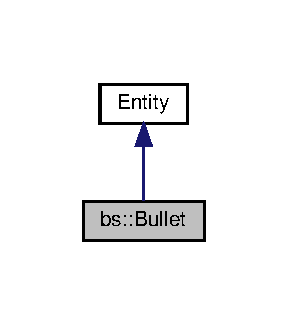
\includegraphics[width=138pt]{classbs_1_1_bullet__inherit__graph}
\end{center}
\end{figure}


Collaboration diagram for bs\+:\+:Bullet\+:
\nopagebreak
\begin{figure}[H]
\begin{center}
\leavevmode
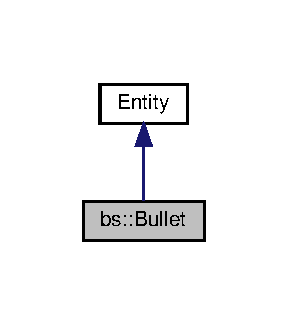
\includegraphics[width=138pt]{classbs_1_1_bullet__coll__graph}
\end{center}
\end{figure}
\subsection*{Public Member Functions}
\begin{DoxyCompactItemize}
\item 
\mbox{\Hypertarget{classbs_1_1_bullet_a43b9135e52be9c24e4ec6f61dbf3d23e}\label{classbs_1_1_bullet_a43b9135e52be9c24e4ec6f61dbf3d23e}} 
{\bfseries Bullet} (const std\+::string file, const std\+::string name\+\_\+, const float speed, float x, float y, float w, float h, int dir)
\item 
\mbox{\Hypertarget{classbs_1_1_bullet_afc39f37eb1ddd13a4603b427fd4a3acc}\label{classbs_1_1_bullet_afc39f37eb1ddd13a4603b427fd4a3acc}} 
void {\bfseries Update} (const sf\+::\+Int64 time)
\item 
\mbox{\Hypertarget{classbs_1_1_bullet_a16b2fc78ea59225d00954a4ae6472f8f}\label{classbs_1_1_bullet_a16b2fc78ea59225d00954a4ae6472f8f}} 
void {\bfseries set\+Alive} (const bool alive\+\_\+status)
\end{DoxyCompactItemize}
\subsection*{Additional Inherited Members}


The documentation for this class was generated from the following files\+:\begin{DoxyCompactItemize}
\item 
Bullet.\+h\item 
Bullet.\+cpp\end{DoxyCompactItemize}

\hypertarget{class_drag_and_drop}{}\section{Drag\+And\+Drop Class Reference}
\label{class_drag_and_drop}\index{Drag\+And\+Drop@{Drag\+And\+Drop}}
\subsection*{Public Member Functions}
\begin{DoxyCompactItemize}
\item 
\mbox{\Hypertarget{class_drag_and_drop_aad31690e074467557cb441c35309533c}\label{class_drag_and_drop_aad31690e074467557cb441c35309533c}} 
{\bfseries Drag\+And\+Drop} (sf\+::\+Render\+Window \&window)
\item 
\mbox{\Hypertarget{class_drag_and_drop_ab6230272a81c91f859d810132ab78475}\label{class_drag_and_drop_ab6230272a81c91f859d810132ab78475}} 
void {\bfseries Move\+Mouse} (sf\+::\+Render\+Window \&window)
\item 
\mbox{\Hypertarget{class_drag_and_drop_a988d844560b5cc186b19b0a1d01ba5f6}\label{class_drag_and_drop_a988d844560b5cc186b19b0a1d01ba5f6}} 
void {\bfseries Main\+Effect} (sf\+::\+Event \&event, \hyperlink{class_player}{Player} \&Hero)
\item 
\mbox{\Hypertarget{class_drag_and_drop_a9c7dc3f6e9ed4207e620d72da5cfd24a}\label{class_drag_and_drop_a9c7dc3f6e9ed4207e620d72da5cfd24a}} 
void {\bfseries Action} (\hyperlink{class_player}{Player} \&Hero)
\item 
\mbox{\Hypertarget{class_drag_and_drop_a2a08096bda61d65d0065a36914473768}\label{class_drag_and_drop_a2a08096bda61d65d0065a36914473768}} 
void {\bfseries Set\+Vectors} (sf\+::\+Render\+Window \&window)
\item 
\mbox{\Hypertarget{class_drag_and_drop_aeac40553c39889501ef8b27964835c90}\label{class_drag_and_drop_aeac40553c39889501ef8b27964835c90}} 
void {\bfseries Select} (sf\+::\+Render\+Window \&window, sf\+::\+Event \&event, \hyperlink{class_player}{Player} \&Hero)
\item 
\mbox{\Hypertarget{class_drag_and_drop_a99a6ff107cc3495bf0526d585dc6aa63}\label{class_drag_and_drop_a99a6ff107cc3495bf0526d585dc6aa63}} 
void {\bfseries Rpg} (sf\+::\+Event \&event, \hyperlink{class_player}{Player} \&Hero)
\item 
\mbox{\Hypertarget{class_drag_and_drop_ad15d9ee16278025b418b9d468e3b5250}\label{class_drag_and_drop_ad15d9ee16278025b418b9d468e3b5250}} 
void {\bfseries Move\+Sprite} (\hyperlink{class_player}{Player} \&Hero, sf\+::\+Int64 \&time)
\item 
\mbox{\Hypertarget{class_drag_and_drop_ad800ef9848505746c7e8479bfe57dd70}\label{class_drag_and_drop_ad800ef9848505746c7e8479bfe57dd70}} 
void {\bfseries Drop\+Color} (\hyperlink{class_player}{Player} \&Hero, sf\+::\+Event \&event)
\item 
\mbox{\Hypertarget{class_drag_and_drop_a57e90c907e9037dc80bfef7c755e8840}\label{class_drag_and_drop_a57e90c907e9037dc80bfef7c755e8840}} 
void {\bfseries Rotate} (\hyperlink{class_player}{Player} \&Hero)
\end{DoxyCompactItemize}


The documentation for this class was generated from the following files\+:\begin{DoxyCompactItemize}
\item 
Drag\+And\+Drop.\+h\item 
Drag\+And\+Drop.\+cpp\end{DoxyCompactItemize}

\hypertarget{class_enemy}{}\section{Enemy Class Reference}
\label{class_enemy}\index{Enemy@{Enemy}}


Inheritance diagram for Enemy\+:
\nopagebreak
\begin{figure}[H]
\begin{center}
\leavevmode
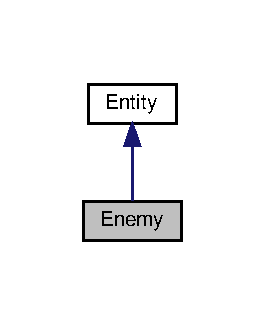
\includegraphics[width=127pt]{class_enemy__inherit__graph}
\end{center}
\end{figure}


Collaboration diagram for Enemy\+:
\nopagebreak
\begin{figure}[H]
\begin{center}
\leavevmode
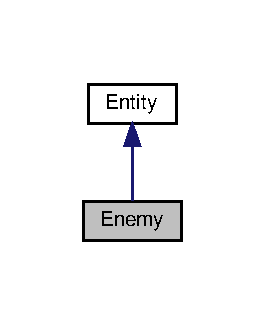
\includegraphics[width=127pt]{class_enemy__coll__graph}
\end{center}
\end{figure}
\subsection*{Public Member Functions}
\begin{DoxyCompactItemize}
\item 
\mbox{\Hypertarget{class_enemy_a7b9b492eeac5b510228c2c0d8757706f}\label{class_enemy_a7b9b492eeac5b510228c2c0d8757706f}} 
{\bfseries Enemy} (const std\+::string file, std\+::string name\+\_\+, float x, float y, float w, float h, float start\+Timer)
\item 
\mbox{\Hypertarget{class_enemy_abe881a77eff5534c8bb024c168ca38d6}\label{class_enemy_abe881a77eff5534c8bb024c168ca38d6}} 
void {\bfseries Check\+Collision} (\hyperlink{class_map}{Map} \&map, float dx\+\_\+, float dy\+\_\+)
\item 
\mbox{\Hypertarget{class_enemy_a66d6e2b40b06aae79cd3fea45d5f48f9}\label{class_enemy_a66d6e2b40b06aae79cd3fea45d5f48f9}} 
void {\bfseries Update} (\hyperlink{class_map}{Map} \&map, sf\+::\+Int64 time)
\item 
\mbox{\Hypertarget{class_enemy_a73dcc317c01af52b3c97aa083d65de47}\label{class_enemy_a73dcc317c01af52b3c97aa083d65de47}} 
void {\bfseries Set\+Next} (\hyperlink{class_enemy}{Enemy} $\ast$next\+\_\+en)
\item 
\mbox{\Hypertarget{class_enemy_a3cf51ab0fd168ec3dc8bbeaebcb96928}\label{class_enemy_a3cf51ab0fd168ec3dc8bbeaebcb96928}} 
void {\bfseries Reduce\+HP} ()
\item 
\mbox{\Hypertarget{class_enemy_a17c7a835e1ef65b5e181b53aa93c07e3}\label{class_enemy_a17c7a835e1ef65b5e181b53aa93c07e3}} 
void {\bfseries Destruct} ()
\item 
\mbox{\Hypertarget{class_enemy_a3fb49a47746dc5396f0bc0b3081bf79f}\label{class_enemy_a3fb49a47746dc5396f0bc0b3081bf79f}} 
void {\bfseries illustrate\+Damage} ()
\item 
\mbox{\Hypertarget{class_enemy_a03fcd0d6de2ef83669f381701f86d788}\label{class_enemy_a03fcd0d6de2ef83669f381701f86d788}} 
void {\bfseries Set\+Attacked} ()
\item 
\mbox{\Hypertarget{class_enemy_a4bd03366a45b265d91bb167007a38132}\label{class_enemy_a4bd03366a45b265d91bb167007a38132}} 
void {\bfseries Display\+Damage} (const sf\+::\+Int64 time)
\item 
\mbox{\Hypertarget{class_enemy_a6562574a2090a4e63322dd94485603d5}\label{class_enemy_a6562574a2090a4e63322dd94485603d5}} 
void {\bfseries player\+Collision} (const \hyperlink{class_player}{Player} \&Hero)
\item 
\mbox{\Hypertarget{class_enemy_a92203a84314188cd99c95390e0c78df4}\label{class_enemy_a92203a84314188cd99c95390e0c78df4}} 
void {\bfseries add\+Bullet} (const sf\+::\+Int64 \&time)
\item 
\mbox{\Hypertarget{class_enemy_a1bcb2bfb62fa715feee98525fd541eaa}\label{class_enemy_a1bcb2bfb62fa715feee98525fd541eaa}} 
void {\bfseries generate\+Dir} (const sf\+::\+Int64 \&time)
\item 
\mbox{\Hypertarget{class_enemy_a261b7c164def36e1badf7ad6f5081856}\label{class_enemy_a261b7c164def36e1badf7ad6f5081856}} 
void {\bfseries follow\+Player} (const sf\+::\+Vector2f \&pl\+Pos)
\item 
\mbox{\Hypertarget{class_enemy_a8487c5726369ecf9d54d5da7320e7d53}\label{class_enemy_a8487c5726369ecf9d54d5da7320e7d53}} 
const sf\+::\+Vector2f \& {\bfseries get\+Coord} ()
\item 
\mbox{\Hypertarget{class_enemy_ac58ecd2844e84278305739188abb0ed5}\label{class_enemy_ac58ecd2844e84278305739188abb0ed5}} 
const sf\+::\+Vector2i {\bfseries get\+Size} () const
\item 
\mbox{\Hypertarget{class_enemy_a8404c22e8b03b56be9ad61738f6524e0}\label{class_enemy_a8404c22e8b03b56be9ad61738f6524e0}} 
\hyperlink{class_enemy}{Enemy} $\ast$ {\bfseries Get\+Next} ()
\item 
\mbox{\Hypertarget{class_enemy_ab94c4bf66e1ec983e6d1fad9daf94c04}\label{class_enemy_ab94c4bf66e1ec983e6d1fad9daf94c04}} 
bool {\bfseries Is\+Attacked} (const sf\+::\+Vector2f \&pl\+Pos, const float distance)
\item 
\mbox{\Hypertarget{class_enemy_aa0e5bf304aede0e04c5b3ff7c4c4008b}\label{class_enemy_aa0e5bf304aede0e04c5b3ff7c4c4008b}} 
bool {\bfseries is\+Time\+Bullet} (const sf\+::\+Int64 time)
\item 
\mbox{\Hypertarget{class_enemy_afefdcb8e4d8947dd4da80d2ceebb1219}\label{class_enemy_afefdcb8e4d8947dd4da80d2ceebb1219}} 
const float {\bfseries get\+HP} () const
\item 
\mbox{\Hypertarget{class_enemy_a2e588a943b52172b117d768b1311681b}\label{class_enemy_a2e588a943b52172b117d768b1311681b}} 
const int {\bfseries get\+Dir} () const
\end{DoxyCompactItemize}
\subsection*{Additional Inherited Members}


The documentation for this class was generated from the following files\+:\begin{DoxyCompactItemize}
\item 
Enemy.\+h\item 
Enemy.\+cpp\end{DoxyCompactItemize}

\hypertarget{class_engine}{}\section{Engine Class Reference}
\label{class_engine}\index{Engine@{Engine}}
\subsection*{Public Member Functions}
\begin{DoxyCompactItemize}
\item 
\mbox{\Hypertarget{class_engine_a1a210cf30d6bd330b3649439ecd6d6cc}\label{class_engine_a1a210cf30d6bd330b3649439ecd6d6cc}} 
void {\bfseries run} ()
\end{DoxyCompactItemize}


The documentation for this class was generated from the following file\+:\begin{DoxyCompactItemize}
\item 
Game.\+cpp\end{DoxyCompactItemize}

\hypertarget{class_entity}{}\section{Entity Class Reference}
\label{class_entity}\index{Entity@{Entity}}


Inheritance diagram for Entity\+:
\nopagebreak
\begin{figure}[H]
\begin{center}
\leavevmode
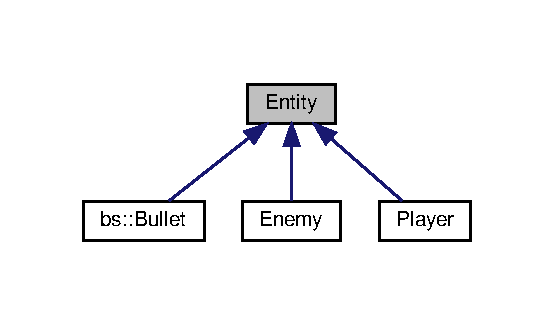
\includegraphics[width=266pt]{class_entity__inherit__graph}
\end{center}
\end{figure}
\subsection*{Public Member Functions}
\begin{DoxyCompactItemize}
\item 
\mbox{\Hypertarget{class_entity_adeafb102a65222ffe3f3764c80fb40be}\label{class_entity_adeafb102a65222ffe3f3764c80fb40be}} 
{\bfseries Entity} (const std\+::string file, const std\+::string name\+\_\+, float x, float y, float w, float h)
\item 
\mbox{\Hypertarget{class_entity_a621c677db785136913ee34889f2f535b}\label{class_entity_a621c677db785136913ee34889f2f535b}} 
void {\bfseries set\+Rotate} (const float value)
\item 
\mbox{\Hypertarget{class_entity_ac5987db2dd874b3df2428196513766e4}\label{class_entity_ac5987db2dd874b3df2428196513766e4}} 
void {\bfseries set\+Color} (const sf\+::\+Color \&color)
\item 
\mbox{\Hypertarget{class_entity_ad42cfa8f3263d6fadd2b6546c4ac5459}\label{class_entity_ad42cfa8f3263d6fadd2b6546c4ac5459}} 
void {\bfseries set\+Origin} (const float x, const float y)
\item 
\mbox{\Hypertarget{class_entity_ab634ca7ef80f912d4da76f341e28b241}\label{class_entity_ab634ca7ef80f912d4da76f341e28b241}} 
void {\bfseries set\+Position} (const float x, const float y)
\item 
\mbox{\Hypertarget{class_entity_af879ce682a20c6c2d270ffd841cf7c26}\label{class_entity_af879ce682a20c6c2d270ffd841cf7c26}} 
void {\bfseries set\+Texture\+Rect} (const sf\+::\+Int\+Rect \&rect)
\item 
\mbox{\Hypertarget{class_entity_a0e2e68071fbe4490a619b4985e643d3b}\label{class_entity_a0e2e68071fbe4490a619b4985e643d3b}} 
void {\bfseries set\+Texture} (sf\+::\+Texture \&texture)
\item 
\mbox{\Hypertarget{class_entity_afd6064663f62605b34859eb9adc6b460}\label{class_entity_afd6064663f62605b34859eb9adc6b460}} 
void {\bfseries set\+Scale} (const float factorX, const float factorY)
\item 
\mbox{\Hypertarget{class_entity_a1309341dd268af435449b5031ff0a06d}\label{class_entity_a1309341dd268af435449b5031ff0a06d}} 
virtual void {\bfseries draw} (sf\+::\+Render\+Window \&window)
\item 
\mbox{\Hypertarget{class_entity_ad47c4683fbc9fb11e2712c7c6b8944c7}\label{class_entity_ad47c4683fbc9fb11e2712c7c6b8944c7}} 
const sf\+::\+Vector2f {\bfseries get\+Position} ()
\item 
\mbox{\Hypertarget{class_entity_a15314da91491df7bca1940a3792799b7}\label{class_entity_a15314da91491df7bca1940a3792799b7}} 
const sf\+::\+Sprite {\bfseries get\+Sprite} () const
\item 
\mbox{\Hypertarget{class_entity_a1047dbb55741460c35c5f59b14420dda}\label{class_entity_a1047dbb55741460c35c5f59b14420dda}} 
const bool {\bfseries get\+Global\+Bounds} (const sf\+::\+Vector2f \&vec) const
\item 
\mbox{\Hypertarget{class_entity_adb4d323c82a9d425fecb4fddcff24b79}\label{class_entity_adb4d323c82a9d425fecb4fddcff24b79}} 
const bool {\bfseries is\+Alive} () const
\end{DoxyCompactItemize}
\subsection*{Public Attributes}
\begin{DoxyCompactItemize}
\item 
\mbox{\Hypertarget{class_entity_a7da0acdf92377bac590ac3fbfb6b496f}\label{class_entity_a7da0acdf92377bac590ac3fbfb6b496f}} 
float {\bfseries Heatpoints}
\item 
\mbox{\Hypertarget{class_entity_a906ea40949afeba12aabef52d7b67587}\label{class_entity_a906ea40949afeba12aabef52d7b67587}} 
sf\+::\+Vector2f {\bfseries Pos}
\item 
\mbox{\Hypertarget{class_entity_a8f987588c24a29e6f0d8cdc9dee1a0a7}\label{class_entity_a8f987588c24a29e6f0d8cdc9dee1a0a7}} 
float {\bfseries Speed}
\item 
\mbox{\Hypertarget{class_entity_abfa9047e1fe7b824fdd837b127513c14}\label{class_entity_abfa9047e1fe7b824fdd837b127513c14}} 
float {\bfseries Width}
\item 
\mbox{\Hypertarget{class_entity_a1f6e7c50981f916434f78b614d09da11}\label{class_entity_a1f6e7c50981f916434f78b614d09da11}} 
float {\bfseries Height}
\item 
\mbox{\Hypertarget{class_entity_a75b5a55635eb07ca229519553137059f}\label{class_entity_a75b5a55635eb07ca229519553137059f}} 
sf\+::\+Int64 {\bfseries Timer}
\item 
\mbox{\Hypertarget{class_entity_a9591c4a913f8348715e9a84d957a8b93}\label{class_entity_a9591c4a913f8348715e9a84d957a8b93}} 
bool {\bfseries Alive}
\item 
\mbox{\Hypertarget{class_entity_a4eeb3d53f6e52112f99145a5cdd7d03d}\label{class_entity_a4eeb3d53f6e52112f99145a5cdd7d03d}} 
bool {\bfseries Is\+Move}
\item 
\mbox{\Hypertarget{class_entity_a2f43af776613b10c5680ea852c78c931}\label{class_entity_a2f43af776613b10c5680ea852c78c931}} 
bool {\bfseries On\+Ground}
\item 
\mbox{\Hypertarget{class_entity_ac6bb4eae35563add00a0512fc7856938}\label{class_entity_ac6bb4eae35563add00a0512fc7856938}} 
sf\+::\+Image {\bfseries Image}
\item 
\mbox{\Hypertarget{class_entity_ad2bef26f8eef4c3c1c9f5830a1cc16d9}\label{class_entity_ad2bef26f8eef4c3c1c9f5830a1cc16d9}} 
sf\+::\+Texture {\bfseries Texture}
\item 
\mbox{\Hypertarget{class_entity_ae8f30f7e882096be1fe49167a16d8611}\label{class_entity_ae8f30f7e882096be1fe49167a16d8611}} 
std\+::string {\bfseries Name}
\item 
\mbox{\Hypertarget{class_entity_a45a52286e7651da8796110069dd31b4b}\label{class_entity_a45a52286e7651da8796110069dd31b4b}} 
std\+::string {\bfseries File}
\item 
\mbox{\Hypertarget{class_entity_a182c63e0b0bedf2159e47b019d769ec4}\label{class_entity_a182c63e0b0bedf2159e47b019d769ec4}} 
float {\bfseries dx}
\item 
\mbox{\Hypertarget{class_entity_ade4d0d757640434826ba88607f1af535}\label{class_entity_ade4d0d757640434826ba88607f1af535}} 
float {\bfseries dy}
\end{DoxyCompactItemize}


The documentation for this class was generated from the following files\+:\begin{DoxyCompactItemize}
\item 
Entity.\+h\item 
Entity.\+cpp\end{DoxyCompactItemize}

\hypertarget{class_game_object}{}\section{Game\+Object Class Reference}
\label{class_game_object}\index{Game\+Object@{Game\+Object}}
\subsection*{Public Member Functions}
\begin{DoxyCompactItemize}
\item 
\mbox{\Hypertarget{class_game_object_ad3ac1deac50048cf7a1a19eb0e61ad26}\label{class_game_object_ad3ac1deac50048cf7a1a19eb0e61ad26}} 
void {\bfseries Draw} ()
\item 
\mbox{\Hypertarget{class_game_object_ab4436b570af026dae6007f44839bd8e5}\label{class_game_object_ab4436b570af026dae6007f44839bd8e5}} 
void {\bfseries Move} ()
\item 
\mbox{\Hypertarget{class_game_object_a000bddf0e0dfb1bbb0f16951cc78d7f1}\label{class_game_object_a000bddf0e0dfb1bbb0f16951cc78d7f1}} 
void {\bfseries Collide} (phystech $\ast$that)
\end{DoxyCompactItemize}
\subsection*{Public Attributes}
\begin{DoxyCompactItemize}
\item 
\mbox{\Hypertarget{class_game_object_afddac54595d19a925bd6346769652abb}\label{class_game_object_afddac54595d19a925bd6346769652abb}} 
std\+::vector$<$ double $>$ {\bfseries position}
\item 
\mbox{\Hypertarget{class_game_object_a26563582dc9aed0a6faa15b33618c766}\label{class_game_object_a26563582dc9aed0a6faa15b33618c766}} 
std\+::vector$<$ double $>$ {\bfseries velocity}
\item 
\mbox{\Hypertarget{class_game_object_a0e640ab7f9c82c41728e88079f00af1a}\label{class_game_object_a0e640ab7f9c82c41728e88079f00af1a}} 
std\+::vector$<$ double $>$ {\bfseries acceleration}
\item 
\mbox{\Hypertarget{class_game_object_a2db2ed0382dcd0bd36a6e01afd49fe36}\label{class_game_object_a2db2ed0382dcd0bd36a6e01afd49fe36}} 
std\+::vector$<$ double $>$ {\bfseries mass}
\item 
\mbox{\Hypertarget{class_game_object_a70da55d7631b506a91309249f9eb2e0f}\label{class_game_object_a70da55d7631b506a91309249f9eb2e0f}} 
sf\+::\+Sprite {\bfseries spr}
\end{DoxyCompactItemize}


The documentation for this class was generated from the following file\+:\begin{DoxyCompactItemize}
\item 
Game.\+cpp\end{DoxyCompactItemize}

\hypertarget{struct_layer}{}\section{Layer Struct Reference}
\label{struct_layer}\index{Layer@{Layer}}
\subsection*{Public Attributes}
\begin{DoxyCompactItemize}
\item 
\mbox{\Hypertarget{struct_layer_a335b0615d255a1163f1728a9809423e2}\label{struct_layer_a335b0615d255a1163f1728a9809423e2}} 
int {\bfseries opacity}
\item 
\mbox{\Hypertarget{struct_layer_a14ab8b141e54f1e2bfd2a6746c2fc077}\label{struct_layer_a14ab8b141e54f1e2bfd2a6746c2fc077}} 
std\+::vector$<$ sf\+::\+Sprite $>$ {\bfseries tiles}
\end{DoxyCompactItemize}


The documentation for this struct was generated from the following file\+:\begin{DoxyCompactItemize}
\item 
level.\+h\end{DoxyCompactItemize}

\hypertarget{class_level}{}\section{Level Class Reference}
\label{class_level}\index{Level@{Level}}
\subsection*{Public Member Functions}
\begin{DoxyCompactItemize}
\item 
\mbox{\Hypertarget{class_level_a1f10e04fbe066347b35705c01dc0b115}\label{class_level_a1f10e04fbe066347b35705c01dc0b115}} 
bool {\bfseries Load\+From\+File} (std\+::string filename)
\item 
\mbox{\Hypertarget{class_level_aafa37d550b85fed38e0159f5b257807f}\label{class_level_aafa37d550b85fed38e0159f5b257807f}} 
\hyperlink{class_object}{Object} {\bfseries Get\+Object} (std\+::string name)
\item 
\mbox{\Hypertarget{class_level_afdaad3ce4e5188ae855ebda4257ffe8c}\label{class_level_afdaad3ce4e5188ae855ebda4257ffe8c}} 
bool {\bfseries Is\+Solid\+Pixel} (int x, int y)
\item 
\mbox{\Hypertarget{class_level_aca8516e9f864821381f63bdeeb5dc944}\label{class_level_aca8516e9f864821381f63bdeeb5dc944}} 
bool {\bfseries Is\+Solid\+Tile} (int x, int y)
\item 
\mbox{\Hypertarget{class_level_ab49d6a53dd7bac6bba2a7ba83369100e}\label{class_level_ab49d6a53dd7bac6bba2a7ba83369100e}} 
void {\bfseries Move} (int x\+Step, int y\+Step)
\item 
\mbox{\Hypertarget{class_level_a23e3a3c1294d54ddfcd7288ba481aba3}\label{class_level_a23e3a3c1294d54ddfcd7288ba481aba3}} 
void {\bfseries Set\+Drawing\+Bounds} (sf\+::\+Rect$<$ float $>$ bounds)
\item 
\mbox{\Hypertarget{class_level_ae3c2bfbfc60cb52c1945eea100141f32}\label{class_level_ae3c2bfbfc60cb52c1945eea100141f32}} 
void {\bfseries Draw} (sf\+::\+Render\+Window \&window)
\end{DoxyCompactItemize}


The documentation for this class was generated from the following files\+:\begin{DoxyCompactItemize}
\item 
level.\+h\item 
level.\+cpp\end{DoxyCompactItemize}

\hypertarget{class_map}{}\section{Map Class Reference}
\label{class_map}\index{Map@{Map}}
\subsection*{Public Member Functions}
\begin{DoxyCompactItemize}
\item 
\mbox{\Hypertarget{class_map_a1ac0ad9071d24a65b842f0e2dd74d986}\label{class_map_a1ac0ad9071d24a65b842f0e2dd74d986}} 
{\bfseries Map} (const std\+::string file)
\item 
\mbox{\Hypertarget{class_map_a707c89f31c87539009b6e89f57dbe167}\label{class_map_a707c89f31c87539009b6e89f57dbe167}} 
void {\bfseries Load\+Im} ()
\item 
\mbox{\Hypertarget{class_map_a6d9f49662f075fc8848ec3a749a95f00}\label{class_map_a6d9f49662f075fc8848ec3a749a95f00}} 
void {\bfseries Load\+Map} ()
\item 
\mbox{\Hypertarget{class_map_a0b145ae9417d0bea4a410b7fcecf99e1}\label{class_map_a0b145ae9417d0bea4a410b7fcecf99e1}} 
void {\bfseries Set\+Sprite} ()
\item 
\mbox{\Hypertarget{class_map_ae32f5ef95701e0556b6c90994a6457d9}\label{class_map_ae32f5ef95701e0556b6c90994a6457d9}} 
void {\bfseries Draw\+Map} (sf\+::\+Render\+Window \&window)
\item 
\mbox{\Hypertarget{class_map_a6c60ce2101f04b5619efbe6a43f1e2f9}\label{class_map_a6c60ce2101f04b5619efbe6a43f1e2f9}} 
char {\bfseries Get\+Elem\+Map} (unsigned int first, unsigned int second)
\item 
\mbox{\Hypertarget{class_map_a478d85aca5e3af14cf80c8e9bc9d8bca}\label{class_map_a478d85aca5e3af14cf80c8e9bc9d8bca}} 
void {\bfseries Set\+Elem\+Map} (unsigned int first, unsigned int second, char sym)
\item 
\mbox{\Hypertarget{class_map_a4fb6aba33b00688ad1faeb0e1ceec9aa}\label{class_map_a4fb6aba33b00688ad1faeb0e1ceec9aa}} 
void {\bfseries Random\+Generator} (char src, char dest, unsigned int number\+\_\+)
\item 
\mbox{\Hypertarget{class_map_a943e70a9e8a4f1715f2c15b9d93e460b}\label{class_map_a943e70a9e8a4f1715f2c15b9d93e460b}} 
void {\bfseries Generate\+In\+Time} (sf\+::\+Int64 \&timer, sf\+::\+Int64 time, sf\+::\+Int64 period, char src, char dest, unsigned int number\+\_\+)
\end{DoxyCompactItemize}


The documentation for this class was generated from the following files\+:\begin{DoxyCompactItemize}
\item 
Map.\+h\item 
Map.\+cpp\end{DoxyCompactItemize}

\hypertarget{classmenu_1_1_menu}{}\section{menu\+:\+:Menu Class Reference}
\label{classmenu_1_1_menu}\index{menu\+::\+Menu@{menu\+::\+Menu}}
\subsection*{Public Member Functions}
\begin{DoxyCompactItemize}
\item 
\mbox{\Hypertarget{classmenu_1_1_menu_a471c1c981d516b2c921710b9d46b4d64}\label{classmenu_1_1_menu_a471c1c981d516b2c921710b9d46b4d64}} 
{\bfseries Menu} (std\+::size\+\_\+t size,...)
\item 
\mbox{\Hypertarget{classmenu_1_1_menu_a543eab53140ee366c47de0056836d98e}\label{classmenu_1_1_menu_a543eab53140ee366c47de0056836d98e}} 
void {\bfseries set\+Menu\+Num} (int number, \hyperlink{classau_1_1_audio}{au\+::\+Audio} \&audio)
\item 
\mbox{\Hypertarget{classmenu_1_1_menu_a72d4d9a66df79b28dff856046290e7c8}\label{classmenu_1_1_menu_a72d4d9a66df79b28dff856046290e7c8}} 
void {\bfseries set\+Menu\+Status} (const bool status)
\item 
\mbox{\Hypertarget{classmenu_1_1_menu_a15c3d50dbe231b4ea742dbdd3798d182}\label{classmenu_1_1_menu_a15c3d50dbe231b4ea742dbdd3798d182}} 
void {\bfseries set\+Position} (std\+::size\+\_\+t size,...)
\item 
\mbox{\Hypertarget{classmenu_1_1_menu_af4f0954c9afaf67bde64f630705d7034}\label{classmenu_1_1_menu_af4f0954c9afaf67bde64f630705d7034}} 
void {\bfseries set\+Color} (...)
\item 
\mbox{\Hypertarget{classmenu_1_1_menu_a944c3b2c03a066646ad9f34bc29fb7c1}\label{classmenu_1_1_menu_a944c3b2c03a066646ad9f34bc29fb7c1}} 
void {\bfseries draw} (sf\+::\+Render\+Window \&window)
\item 
\mbox{\Hypertarget{classmenu_1_1_menu_a78bbc128a14245fdf727025fcd1a6aca}\label{classmenu_1_1_menu_a78bbc128a14245fdf727025fcd1a6aca}} 
const bool {\bfseries is\+Drawable} () const
\item 
\mbox{\Hypertarget{classmenu_1_1_menu_ac9ecfcb61a15d56f8c3affbcb3398b42}\label{classmenu_1_1_menu_ac9ecfcb61a15d56f8c3affbcb3398b42}} 
const B\+A\+N\+N\+ER {\bfseries get\+Status} () const
\item 
\mbox{\Hypertarget{classmenu_1_1_menu_ad53be26e55cee886dd16aa0b5e0b80cd}\label{classmenu_1_1_menu_ad53be26e55cee886dd16aa0b5e0b80cd}} 
\hyperlink{classmenu_1_1_menu_set}{Menu\+Set} \& {\bfseries get\+Set} (const std\+::size\+\_\+t num)
\end{DoxyCompactItemize}


The documentation for this class was generated from the following files\+:\begin{DoxyCompactItemize}
\item 
Menu.\+h\item 
Menu.\+cpp\end{DoxyCompactItemize}

\hypertarget{classmenu_1_1_menu_set}{}\section{menu\+:\+:Menu\+Set Class Reference}
\label{classmenu_1_1_menu_set}\index{menu\+::\+Menu\+Set@{menu\+::\+Menu\+Set}}
\subsection*{Public Member Functions}
\begin{DoxyCompactItemize}
\item 
\mbox{\Hypertarget{classmenu_1_1_menu_set_ab5c3e7d4860b8d3255235b702b8e2488}\label{classmenu_1_1_menu_set_ab5c3e7d4860b8d3255235b702b8e2488}} 
{\bfseries Menu\+Set} (const std\+::string \&file)
\item 
\mbox{\Hypertarget{classmenu_1_1_menu_set_af05fd419b9d2e95710a465f8ee35ec34}\label{classmenu_1_1_menu_set_af05fd419b9d2e95710a465f8ee35ec34}} 
void {\bfseries draw} (sf\+::\+Render\+Window \&window)
\item 
\mbox{\Hypertarget{classmenu_1_1_menu_set_acec30ab4f92e60902b439833bc2e9a9d}\label{classmenu_1_1_menu_set_acec30ab4f92e60902b439833bc2e9a9d}} 
void {\bfseries set\+Position} (const sf\+::\+Vector2f \&pos)
\item 
\mbox{\Hypertarget{classmenu_1_1_menu_set_a3873b2447f3d76f4e0b211e7bcca3797}\label{classmenu_1_1_menu_set_a3873b2447f3d76f4e0b211e7bcca3797}} 
void {\bfseries set\+Color} (const sf\+::\+Color color)
\end{DoxyCompactItemize}


The documentation for this class was generated from the following files\+:\begin{DoxyCompactItemize}
\item 
Menu.\+h\item 
Menu.\+cpp\end{DoxyCompactItemize}

\hypertarget{class_mission}{}\section{Mission Class Reference}
\label{class_mission}\index{Mission@{Mission}}
\subsection*{Public Member Functions}
\begin{DoxyCompactItemize}
\item 
\mbox{\Hypertarget{class_mission_a740ba1b69124dbb0f70daf74f513305b}\label{class_mission_a740ba1b69124dbb0f70daf74f513305b}} 
{\bfseries Mission} (const std\+::string file\+\_\+\+Kum, const std\+::string file\+\_\+\+Intro)
\item 
\mbox{\Hypertarget{class_mission_ac33b0d9fe70c1b3957ce5b1e8b6c0f3e}\label{class_mission_ac33b0d9fe70c1b3957ce5b1e8b6c0f3e}} 
void {\bfseries Set\+Cur\+Mission} (float coord\+\_\+x)
\item 
\mbox{\Hypertarget{class_mission_a89bbed0549015c07ab3381e32e335a23}\label{class_mission_a89bbed0549015c07ab3381e32e335a23}} 
unsigned int {\bfseries Get\+Cur\+Mission} ()
\item 
\mbox{\Hypertarget{class_mission_ae5383a2bd4c5c3c21ea9eba4c1c46a3a}\label{class_mission_ae5383a2bd4c5c3c21ea9eba4c1c46a3a}} 
std\+::string {\bfseries Get\+Text\+Mission} (unsigned int mission\+\_\+numb)
\item 
\mbox{\Hypertarget{class_mission_acc25406e4bbe28749081eb0a0d81031a}\label{class_mission_acc25406e4bbe28749081eb0a0d81031a}} 
void {\bfseries Load\+Mission} ()
\item 
\mbox{\Hypertarget{class_mission_a67b3876fda2635511f7e24c373e2b6a3}\label{class_mission_a67b3876fda2635511f7e24c373e2b6a3}} 
bool \& {\bfseries Is\+Show} ()
\item 
\mbox{\Hypertarget{class_mission_a11a5f5ac9b25334c5e75d80350f535f7}\label{class_mission_a11a5f5ac9b25334c5e75d80350f535f7}} 
void {\bfseries Set\+Show} (bool value)
\item 
\mbox{\Hypertarget{class_mission_ac2f25c4f3a8fd7bb66d6bce9eb2ca9ae}\label{class_mission_ac2f25c4f3a8fd7bb66d6bce9eb2ca9ae}} 
void {\bfseries Set\+Kum} (float coord\+\_\+x, float coord\+\_\+y)
\item 
\mbox{\Hypertarget{class_mission_a4fcc2cd3642b539229534358ca17efcc}\label{class_mission_a4fcc2cd3642b539229534358ca17efcc}} 
void {\bfseries Draw\+Kum} (sf\+::\+Render\+Window \&window)
\item 
\mbox{\Hypertarget{class_mission_a2568f94df43f8fa470069cc9a1091a94}\label{class_mission_a2568f94df43f8fa470069cc9a1091a94}} 
void {\bfseries Set\+Intro} (float coord\+\_\+x, float coord\+\_\+y)
\item 
\mbox{\Hypertarget{class_mission_ae7bfdc2586760ca48393a22bcf9e774f}\label{class_mission_ae7bfdc2586760ca48393a22bcf9e774f}} 
void {\bfseries Draw\+Intro} (sf\+::\+Render\+Window \&window)
\end{DoxyCompactItemize}


The documentation for this class was generated from the following files\+:\begin{DoxyCompactItemize}
\item 
Mission.\+h\item 
Mission.\+cpp\end{DoxyCompactItemize}

\hypertarget{class_my_view}{}\section{My\+View Class Reference}
\label{class_my_view}\index{My\+View@{My\+View}}
\subsection*{Public Member Functions}
\begin{DoxyCompactItemize}
\item 
\mbox{\Hypertarget{class_my_view_adaba5febb33731c437501caa0be18b75}\label{class_my_view_adaba5febb33731c437501caa0be18b75}} 
sf\+::\+View {\bfseries Get\+Coord\+View} (float xcoord, float ycoord)
\item 
\mbox{\Hypertarget{class_my_view_a4d0cef1553c9329a205c1aa8de764a66}\label{class_my_view_a4d0cef1553c9329a205c1aa8de764a66}} 
sf\+::\+View {\bfseries Scroll\+Map} (sf\+::\+Int64 time)
\item 
\mbox{\Hypertarget{class_my_view_a8ed8988e427222feae35b3d299ded5fe}\label{class_my_view_a8ed8988e427222feae35b3d299ded5fe}} 
void {\bfseries Scroll\+Mouse} (sf\+::\+Window \&window, sf\+::\+Int64 time, const bool is\+Alive)
\end{DoxyCompactItemize}
\subsection*{Public Attributes}
\begin{DoxyCompactItemize}
\item 
\mbox{\Hypertarget{class_my_view_aa7ba3e20e09a2f693012d2279dbb9a1d}\label{class_my_view_aa7ba3e20e09a2f693012d2279dbb9a1d}} 
sf\+::\+View {\bfseries view}
\item 
\mbox{\Hypertarget{class_my_view_ac9e234f611a3db83dfeb342cb821a6dd}\label{class_my_view_ac9e234f611a3db83dfeb342cb821a6dd}} 
sf\+::\+Render\+Window {\bfseries window}
\end{DoxyCompactItemize}


The documentation for this class was generated from the following files\+:\begin{DoxyCompactItemize}
\item 
View.\+h\item 
View.\+cpp\end{DoxyCompactItemize}

\hypertarget{class_object}{}\section{Object Class Reference}
\label{class_object}\index{Object@{Object}}
\subsection*{Public Member Functions}
\begin{DoxyCompactItemize}
\item 
\mbox{\Hypertarget{class_object_a3508bb776edb1139d41c10c1302a532a}\label{class_object_a3508bb776edb1139d41c10c1302a532a}} 
int {\bfseries Get\+Property\+Int} (std\+::string name)
\item 
\mbox{\Hypertarget{class_object_addc3379119fd3cc698ff466c9d371f30}\label{class_object_addc3379119fd3cc698ff466c9d371f30}} 
float {\bfseries Get\+Property\+Float} (std\+::string name)
\item 
\mbox{\Hypertarget{class_object_a3979e6a58390fb4244535f320a3e5db8}\label{class_object_a3979e6a58390fb4244535f320a3e5db8}} 
std\+::string {\bfseries Get\+Property\+String} (std\+::string name)
\end{DoxyCompactItemize}
\subsection*{Public Attributes}
\begin{DoxyCompactItemize}
\item 
\mbox{\Hypertarget{class_object_a24457e0a387492c80594aec7681a2277}\label{class_object_a24457e0a387492c80594aec7681a2277}} 
std\+::string {\bfseries name}
\item 
\mbox{\Hypertarget{class_object_a2f0ab0ca2d98028fd10807a03fcd75e5}\label{class_object_a2f0ab0ca2d98028fd10807a03fcd75e5}} 
std\+::string {\bfseries type}
\item 
\mbox{\Hypertarget{class_object_a800c7b81397ba0e59f2824c8e405ee15}\label{class_object_a800c7b81397ba0e59f2824c8e405ee15}} 
sf\+::\+Rect$<$ int $>$ {\bfseries rect}
\item 
\mbox{\Hypertarget{class_object_af4ca2590a9451ea032eb5aa1f7c799a0}\label{class_object_af4ca2590a9451ea032eb5aa1f7c799a0}} 
std\+::map$<$ std\+::string, std\+::string $>$ {\bfseries properties}
\end{DoxyCompactItemize}


The documentation for this class was generated from the following files\+:\begin{DoxyCompactItemize}
\item 
level.\+h\item 
level.\+cpp\end{DoxyCompactItemize}

\hypertarget{class_player}{}\section{Player Class Reference}
\label{class_player}\index{Player@{Player}}


Inheritance diagram for Player\+:
\nopagebreak
\begin{figure}[H]
\begin{center}
\leavevmode
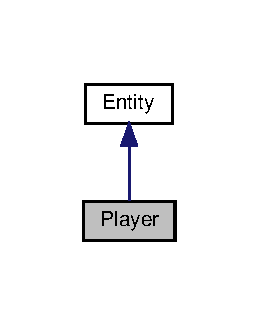
\includegraphics[width=124pt]{class_player__inherit__graph}
\end{center}
\end{figure}


Collaboration diagram for Player\+:
\nopagebreak
\begin{figure}[H]
\begin{center}
\leavevmode
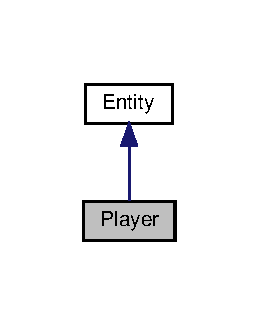
\includegraphics[width=124pt]{class_player__coll__graph}
\end{center}
\end{figure}
\subsection*{Public Member Functions}
\begin{DoxyCompactItemize}
\item 
\mbox{\Hypertarget{class_player_abafd446ede2e1a770374fa14bdb0a4e7}\label{class_player_abafd446ede2e1a770374fa14bdb0a4e7}} 
{\bfseries Player} (const std\+::string file, const std\+::string name, float x, float y, float w, float h)
\item 
\mbox{\Hypertarget{class_player_af5852c410ca00fd6e0f1df220ebd7252}\label{class_player_af5852c410ca00fd6e0f1df220ebd7252}} 
bool {\bfseries Update} (sf\+::\+Int64 time, \hyperlink{class_map}{Map} \&map)
\item 
\mbox{\Hypertarget{class_player_a9ee7c669f1a11cf8e4b05c100450e2b7}\label{class_player_a9ee7c669f1a11cf8e4b05c100450e2b7}} 
bool {\bfseries Get\+Alive} ()
\item 
\mbox{\Hypertarget{class_player_ae5f85a02134fc92697c7fdba20c642f5}\label{class_player_ae5f85a02134fc92697c7fdba20c642f5}} 
bool {\bfseries Set\+Power} (sf\+::\+Int64 time)
\item 
\mbox{\Hypertarget{class_player_a54a908f0d556cb9de705e6084454c15a}\label{class_player_a54a908f0d556cb9de705e6084454c15a}} 
bool {\bfseries Get\+Select} ()
\item 
\mbox{\Hypertarget{class_player_a960f09a55c9150be442a9b8c151179d3}\label{class_player_a960f09a55c9150be442a9b8c151179d3}} 
bool {\bfseries Get\+Move} ()
\item 
\mbox{\Hypertarget{class_player_a41f4db3d836b71b355d84a0cb4317361}\label{class_player_a41f4db3d836b71b355d84a0cb4317361}} 
bool {\bfseries Get\+Hit} () const
\item 
\mbox{\Hypertarget{class_player_a741d3f60b6957c7907b7d7007be642e7}\label{class_player_a741d3f60b6957c7907b7d7007be642e7}} 
bool {\bfseries is\+Bullet\+Attack} (const sf\+::\+Vector2f \&bull\+Pos, const float distance)
\item 
\mbox{\Hypertarget{class_player_af0e6ea79c8e1d2f5994f6c79f2d158bb}\label{class_player_af0e6ea79c8e1d2f5994f6c79f2d158bb}} 
bool {\bfseries Get\+Timer} () const
\item 
\mbox{\Hypertarget{class_player_aa572817a620dedc98ff4634152b12b97}\label{class_player_aa572817a620dedc98ff4634152b12b97}} 
float {\bfseries Get\+CoordX} () const
\item 
\mbox{\Hypertarget{class_player_afe3678c701d5ed81f0c1729a3265b6b3}\label{class_player_afe3678c701d5ed81f0c1729a3265b6b3}} 
float {\bfseries Get\+CoordY} () const
\item 
\mbox{\Hypertarget{class_player_a859e61a326e4700ad455be2efa887af9}\label{class_player_a859e61a326e4700ad455be2efa887af9}} 
float {\bfseries Get\+Speed} () const
\item 
\mbox{\Hypertarget{class_player_ab9b38c788867a135ba1d8fe8e54ed9c7}\label{class_player_ab9b38c788867a135ba1d8fe8e54ed9c7}} 
float {\bfseries Get\+Power} () const
\item 
\mbox{\Hypertarget{class_player_a2fd2366f2ae52f3bf13f6ef3fa81e508}\label{class_player_a2fd2366f2ae52f3bf13f6ef3fa81e508}} 
void {\bfseries Set\+Dir} (int dir)
\item 
\mbox{\Hypertarget{class_player_a2b84b6227dba65e2c5e9a66d0f96e759}\label{class_player_a2b84b6227dba65e2c5e9a66d0f96e759}} 
void {\bfseries Set\+Speed} (float speed)
\item 
\mbox{\Hypertarget{class_player_adb838303b0c98d8f007bebb1a53e12b7}\label{class_player_adb838303b0c98d8f007bebb1a53e12b7}} 
void {\bfseries Interract\+Map} (sf\+::\+Int64 time, \hyperlink{class_map}{Map} \&map)
\item 
\mbox{\Hypertarget{class_player_aea8dbe8f9812a6828c1709972c4c559b}\label{class_player_aea8dbe8f9812a6828c1709972c4c559b}} 
void {\bfseries Set\+HP} (std\+::ostringstream \&Heat\+Points)
\item 
\mbox{\Hypertarget{class_player_a9fac998af5b803e87532df34766d2391}\label{class_player_a9fac998af5b803e87532df34766d2391}} 
void {\bfseries Push\+Score} (std\+::ostringstream \&Score\+String)
\item 
\mbox{\Hypertarget{class_player_a62c904fc9e79a9012cfd449e201554f2}\label{class_player_a62c904fc9e79a9012cfd449e201554f2}} 
void {\bfseries Get\+Air} (std\+::ostringstream \&Score\+Air)
\item 
\mbox{\Hypertarget{class_player_ad92f3ca39bcc0b8739f71659285ea5e6}\label{class_player_ad92f3ca39bcc0b8739f71659285ea5e6}} 
void {\bfseries Push\+Power} (std\+::ostringstream \&Power\+\_\+str)
\item 
\mbox{\Hypertarget{class_player_a84627845c5841d3cc13f95e6972241e6}\label{class_player_a84627845c5841d3cc13f95e6972241e6}} 
void {\bfseries Increase\+Power} (sf\+::\+Int64 time)
\item 
\mbox{\Hypertarget{class_player_acf68380dc8a0481fd60194252b053a3a}\label{class_player_acf68380dc8a0481fd60194252b053a3a}} 
void {\bfseries Set\+Coord} (const float x, const float y)
\item 
\mbox{\Hypertarget{class_player_a265a11fc851ad9c8e4e2a80006ab80d1}\label{class_player_a265a11fc851ad9c8e4e2a80006ab80d1}} 
void {\bfseries Set\+Select} (bool value)
\item 
\mbox{\Hypertarget{class_player_a4460f69d665a8e9bfd65dab4482b834a}\label{class_player_a4460f69d665a8e9bfd65dab4482b834a}} 
void {\bfseries Set\+Move} (bool value)
\item 
\mbox{\Hypertarget{class_player_a711adfffe304ec88e99c94520048c1f4}\label{class_player_a711adfffe304ec88e99c94520048c1f4}} 
void {\bfseries Inc\+Coord} (const float x, const float y)
\item 
\mbox{\Hypertarget{class_player_aba7c42e8bcf1e71d8e326e851537e718}\label{class_player_aba7c42e8bcf1e71d8e326e851537e718}} 
void {\bfseries Purple\+Style} (sf\+::\+Int64 \&time)
\item 
\mbox{\Hypertarget{class_player_a0a2066460adf9ce32fb427aeedcd1d52}\label{class_player_a0a2066460adf9ce32fb427aeedcd1d52}} 
void {\bfseries On\+Fire} (sf\+::\+Int64 \&time)
\item 
\mbox{\Hypertarget{class_player_a1014b3b4371a692f7e64072d1b3bd850}\label{class_player_a1014b3b4371a692f7e64072d1b3bd850}} 
void {\bfseries Set\+Purple} ()
\item 
\mbox{\Hypertarget{class_player_a31cc502c119e0b4646de70bd95fc3710}\label{class_player_a31cc502c119e0b4646de70bd95fc3710}} 
void {\bfseries Set\+Red} ()
\item 
\mbox{\Hypertarget{class_player_ab14c9bfde9a1fd899bd1304ca7c2f7e7}\label{class_player_ab14c9bfde9a1fd899bd1304ca7c2f7e7}} 
void {\bfseries Set\+Hit} ()
\item 
void \hyperlink{class_player_abb881e3cbced276d41fb3d4a3ba4b329}{Hit} (sf\+::\+Int64 \&time, int Y)
\item 
\mbox{\Hypertarget{class_player_aa9dd6c08df215dd4503060f9414b9ae0}\label{class_player_aa9dd6c08df215dd4503060f9414b9ae0}} 
void {\bfseries set\+Bullet\+Attacked} ()
\item 
\mbox{\Hypertarget{class_player_a60debcbc368b0990861bbc2f27838384}\label{class_player_a60debcbc368b0990861bbc2f27838384}} 
void {\bfseries under\+Fire} (const sf\+::\+Int64 \&time)
\item 
\mbox{\Hypertarget{class_player_a169b68ee9a8e5d955675eed2711d5a9a}\label{class_player_a169b68ee9a8e5d955675eed2711d5a9a}} 
unsigned int {\bfseries Get\+Score} ()
\item 
\mbox{\Hypertarget{class_player_a0abe75980955815f82d757f281eeb43f}\label{class_player_a0abe75980955815f82d757f281eeb43f}} 
int {\bfseries Get\+Dir} () const
\item 
\mbox{\Hypertarget{class_player_a404208da6ae6ca92a6c66ef391fcd5cd}\label{class_player_a404208da6ae6ca92a6c66ef391fcd5cd}} 
const sf\+::\+Vector2f \& {\bfseries Get\+Pos} () const
\end{DoxyCompactItemize}
\subsection*{Public Attributes}
\begin{DoxyCompactItemize}
\item 
\mbox{\Hypertarget{class_player_aa71a31c2f38eae8aa3d5c6c764e1cfd1}\label{class_player_aa71a31c2f38eae8aa3d5c6c764e1cfd1}} 
const float {\bfseries n\+\_\+speed} = 0.\+2f
\end{DoxyCompactItemize}


\subsection{Member Function Documentation}
\mbox{\Hypertarget{class_player_abb881e3cbced276d41fb3d4a3ba4b329}\label{class_player_abb881e3cbced276d41fb3d4a3ba4b329}} 
\index{Player@{Player}!Hit@{Hit}}
\index{Hit@{Hit}!Player@{Player}}
\subsubsection{\texorpdfstring{Hit()}{Hit()}}
{\footnotesize\ttfamily void Player\+::\+Hit (\begin{DoxyParamCaption}\item[{sf\+::\+Int64 \&}]{time,  }\item[{int}]{Y }\end{DoxyParamCaption})}

maybe equals 

The documentation for this class was generated from the following files\+:\begin{DoxyCompactItemize}
\item 
Player.\+h\item 
Player.\+cpp\end{DoxyCompactItemize}

\hypertarget{classbs_1_1_pool_bullets}{}\section{bs\+:\+:Pool\+Bullets Class Reference}
\label{classbs_1_1_pool_bullets}\index{bs\+::\+Pool\+Bullets@{bs\+::\+Pool\+Bullets}}
\subsection*{Public Member Functions}
\begin{DoxyCompactItemize}
\item 
\mbox{\Hypertarget{classbs_1_1_pool_bullets_a9d0c69bfd2279e0151ed28439bb53d36}\label{classbs_1_1_pool_bullets_a9d0c69bfd2279e0151ed28439bb53d36}} 
{\bfseries Pool\+Bullets} (std\+::size\+\_\+t size)
\item 
void \hyperlink{classbs_1_1_pool_bullets_a000d643a8fbe7445fef483a474f280f2}{player\+Collision} (\hyperlink{class_player}{Player} \&hero)
\item 
\mbox{\Hypertarget{classbs_1_1_pool_bullets_af7943a4ef9e310f49c5f4843790dd2f4}\label{classbs_1_1_pool_bullets_af7943a4ef9e310f49c5f4843790dd2f4}} 
void {\bfseries enemy\+Collision} (\hyperlink{class_enemy}{Enemy} $\ast$enemy)
\item 
\mbox{\Hypertarget{classbs_1_1_pool_bullets_a014b33cf9f98d78fbd6f99e5ed433287}\label{classbs_1_1_pool_bullets_a014b33cf9f98d78fbd6f99e5ed433287}} 
void {\bfseries add\+Bullet} (const sf\+::\+Vector2f \&en\+Pos, const std\+::string file, const std\+::string name\+\_\+, const float speed, const int dir)
\item 
\mbox{\Hypertarget{classbs_1_1_pool_bullets_a69c5a604921b0d7c6024d605b8b0b6ff}\label{classbs_1_1_pool_bullets_a69c5a604921b0d7c6024d605b8b0b6ff}} 
void {\bfseries Update} (const sf\+::\+Int64 time)
\item 
\mbox{\Hypertarget{classbs_1_1_pool_bullets_a47595b6fc041a91f71df69d750f61545}\label{classbs_1_1_pool_bullets_a47595b6fc041a91f71df69d750f61545}} 
void {\bfseries draw} (sf\+::\+Render\+Window \&window)
\item 
\mbox{\Hypertarget{classbs_1_1_pool_bullets_a99bdbe126b10e249e06dd23d1daff76d}\label{classbs_1_1_pool_bullets_a99bdbe126b10e249e06dd23d1daff76d}} 
std\+::size\+\_\+t {\bfseries get\+Size} ()
\end{DoxyCompactItemize}


\subsection{Member Function Documentation}
\mbox{\Hypertarget{classbs_1_1_pool_bullets_a000d643a8fbe7445fef483a474f280f2}\label{classbs_1_1_pool_bullets_a000d643a8fbe7445fef483a474f280f2}} 
\index{bs\+::\+Pool\+Bullets@{bs\+::\+Pool\+Bullets}!player\+Collision@{player\+Collision}}
\index{player\+Collision@{player\+Collision}!bs\+::\+Pool\+Bullets@{bs\+::\+Pool\+Bullets}}
\subsubsection{\texorpdfstring{player\+Collision()}{playerCollision()}}
{\footnotesize\ttfamily void bs\+::\+Pool\+Bullets\+::player\+Collision (\begin{DoxyParamCaption}\item[{\hyperlink{class_player}{Player} \&}]{hero }\end{DoxyParamCaption})}

!! 

The documentation for this class was generated from the following files\+:\begin{DoxyCompactItemize}
\item 
Pool\+Bullets.\+h\item 
Pool\+Bullets.\+cpp\end{DoxyCompactItemize}

\hypertarget{class_pool_enemies}{}\section{Pool\+Enemies Class Reference}
\label{class_pool_enemies}\index{Pool\+Enemies@{Pool\+Enemies}}
\subsection*{Public Member Functions}
\begin{DoxyCompactItemize}
\item 
\mbox{\Hypertarget{class_pool_enemies_a3dc2f638ddfe5961f9d19690ce8ffc42}\label{class_pool_enemies_a3dc2f638ddfe5961f9d19690ce8ffc42}} 
{\bfseries Pool\+Enemies} (const size\+\_\+t size, const std\+::string file, std\+::string name\+\_\+, float x, float y, float w, float h)
\item 
\mbox{\Hypertarget{class_pool_enemies_a230f6d6152342974d814da58009826ea}\label{class_pool_enemies_a230f6d6152342974d814da58009826ea}} 
void {\bfseries Init} (const std\+::string file, std\+::string name\+\_\+, float x, float y, float w, float h)
\item 
\mbox{\Hypertarget{class_pool_enemies_abd7f45866a211be06d9ff07f00a453d4}\label{class_pool_enemies_abd7f45866a211be06d9ff07f00a453d4}} 
void {\bfseries Create} (\hyperlink{class_enemy}{Enemy} $\ast$enemy, const std\+::string file, std\+::string name\+\_\+, float x, float y, float w, float h)
\item 
\mbox{\Hypertarget{class_pool_enemies_aa4d6670db20d28b1425573a69dce6cd3}\label{class_pool_enemies_aa4d6670db20d28b1425573a69dce6cd3}} 
const size\+\_\+t {\bfseries Get\+Size} ()
\item 
\mbox{\Hypertarget{class_pool_enemies_ac00ab90555d06ab26e07f6679043b759}\label{class_pool_enemies_ac00ab90555d06ab26e07f6679043b759}} 
void {\bfseries Draw\+Pool} (sf\+::\+Render\+Window \&window, const sf\+::\+Int64 time)
\item 
\mbox{\Hypertarget{class_pool_enemies_a96a7fe66f07aed92fae70b53015f3a2f}\label{class_pool_enemies_a96a7fe66f07aed92fae70b53015f3a2f}} 
void {\bfseries Print\+Position} ()
\item 
\mbox{\Hypertarget{class_pool_enemies_ac23a8dd2bc0dfa85317e44ec6a1680a9}\label{class_pool_enemies_ac23a8dd2bc0dfa85317e44ec6a1680a9}} 
void {\bfseries Update} (\hyperlink{class_map}{Map} \&map, sf\+::\+Int64 time, const \hyperlink{class_player}{Player} \&Hero)
\item 
\mbox{\Hypertarget{class_pool_enemies_a6c34f306bef5f07396d6b2a0afc33540}\label{class_pool_enemies_a6c34f306bef5f07396d6b2a0afc33540}} 
void {\bfseries is\+Attacked} (const \hyperlink{class_player}{Player} \&Hero)
\item 
\mbox{\Hypertarget{class_pool_enemies_a82638c91745fa4d84425261547543e7e}\label{class_pool_enemies_a82638c91745fa4d84425261547543e7e}} 
void {\bfseries add\+Bullet} (\hyperlink{classbs_1_1_pool_bullets}{bs\+::\+Pool\+Bullets} \&pool\+Bullets, const std\+::string file, const std\+::string name\+\_\+, const float speed, const sf\+::\+Int64 time, \hyperlink{classau_1_1_audio}{au\+::\+Audio} \&audio)
\item 
\mbox{\Hypertarget{class_pool_enemies_ae15fce84d594589152deaabf8dc166bf}\label{class_pool_enemies_ae15fce84d594589152deaabf8dc166bf}} 
void {\bfseries bullet\+Collision} (\hyperlink{classbs_1_1_pool_bullets}{bs\+::\+Pool\+Bullets} \&b\+Pool)
\item 
\mbox{\Hypertarget{class_pool_enemies_ad5312d398eaa044a92cc5fe52ac34d42}\label{class_pool_enemies_ad5312d398eaa044a92cc5fe52ac34d42}} 
const sf\+::\+Vector2i {\bfseries get\+Size\+Enemies} () const
\item 
\mbox{\Hypertarget{class_pool_enemies_ab35e745455dd4778ae8b121af7c522e1}\label{class_pool_enemies_ab35e745455dd4778ae8b121af7c522e1}} 
const bool {\bfseries is\+Pool\+Alive} () const
\end{DoxyCompactItemize}


The documentation for this class was generated from the following files\+:\begin{DoxyCompactItemize}
\item 
Pool\+Enemies.\+h\item 
Pool\+Enemies.\+cpp\end{DoxyCompactItemize}

\hypertarget{class_text}{}\section{Text Class Reference}
\label{class_text}\index{Text@{Text}}
\subsection*{Public Member Functions}
\begin{DoxyCompactItemize}
\item 
\mbox{\Hypertarget{class_text_a3e37b942e6e90263c69d9355ae7ebb63}\label{class_text_a3e37b942e6e90263c69d9355ae7ebb63}} 
{\bfseries Text} (sf\+::\+Font \&font, sf\+::\+Text \&text, const sf\+::\+Color color, sf\+::\+Text\+::\+Style style, std\+::string \&str, unsigned int size)
\item 
\mbox{\Hypertarget{class_text_a34e2dab4f8a10f62f4da0d4eb55011b7}\label{class_text_a34e2dab4f8a10f62f4da0d4eb55011b7}} 
void {\bfseries Draw} (\hyperlink{class_my_view}{My\+View} \&View, sf\+::\+Render\+Window \&window, int correct\+\_\+x, int correct\+\_\+y)
\item 
\mbox{\Hypertarget{class_text_a72f85268a2666e30819a8b87490beb50}\label{class_text_a72f85268a2666e30819a8b87490beb50}} 
void {\bfseries Print} ()
\item 
\mbox{\Hypertarget{class_text_a5aeb9e86c2fba5f36b1d5520e68a510d}\label{class_text_a5aeb9e86c2fba5f36b1d5520e68a510d}} 
{\footnotesize template$<$typename T $>$ }\\void {\bfseries Push\+Str} (T value)
\item 
\mbox{\Hypertarget{class_text_af8c9bb8280b916276c3c979487cf980e}\label{class_text_af8c9bb8280b916276c3c979487cf980e}} 
void {\bfseries Prepare\+To\+Draw} (\hyperlink{class_my_view}{My\+View} \&View, int correct\+\_\+x, int correct\+\_\+y)
\item 
\mbox{\Hypertarget{class_text_ab4091f56a59b11e1a6304a909acff0a1}\label{class_text_ab4091f56a59b11e1a6304a909acff0a1}} 
std\+::ostringstream \& {\bfseries Get\+Stream} ()
\item 
\mbox{\Hypertarget{class_text_af1fa7ee2429a16ce75480d0e8197d0b5}\label{class_text_af1fa7ee2429a16ce75480d0e8197d0b5}} 
sf\+::\+Text \& {\bfseries Get\+Text} ()
\end{DoxyCompactItemize}


The documentation for this class was generated from the following files\+:\begin{DoxyCompactItemize}
\item 
Text.\+h\item 
Text.\+cpp\end{DoxyCompactItemize}

%--- End generated contents ---

% Index
\backmatter
\newpage
\phantomsection
\clearemptydoublepage
\addcontentsline{toc}{chapter}{Index}
\printindex

\end{document}
